\documentclass[journal]{IEEEtran}
\usepackage[utf8]{inputenc}

\title{DDM Muscima Note Recognition}
\author{Federico Magnolfi\\Stiven Metaj}
\date{February 2019}

\usepackage{xcolor,soul,framed} %,caption
\colorlet{shadecolor}{yellow}
\usepackage[pdftex]{graphicx}
\graphicspath{{../pdf/}{../jpeg/}}
\DeclareGraphicsExtensions{.pdf,.jpeg,.png}
\usepackage[cmex10]{amsmath}
\usepackage{array}
\usepackage{mdwmath}
\usepackage{mdwtab}
\usepackage{eqparbox}
\usepackage{url}
\usepackage{float}




%=== TITLE & AUTHORS ====================================================================
\begin{document}
	\bstctlcite{IEEEexample:BSTcontrol}
	\title{MNR: MUSCIMA Note Recognition.\\ Using Faster R-CNN on handwritten music dataset.}
	\author{Federico Magnolfi,~\IEEEmembership{federico.magnolfi2@stud.unifi.it}\\
		Stiven Metaj,~\IEEEmembership{stiven.metaj@mail.polimi.it}% <-this % stops a space
	}  
	
	% The paper headers
	\markboth{}{}
	
	
	% ====================================================================
	\maketitle
	
	
	
	% === ABSTRACT ====================================================================
	% =================================================================================
	\begin{abstract}
		%\boldmath
		This paper presents a project about the use of Region-based Deep Learning methods to perform Optical Music Recognition (OMR) on handwritten music images. The choice of a dataset to manipulate is critical; in this case, the new MUSCIMA++ (a subset of CVCMUSCIMA) is chosen: it offers primitives and high-level notation objects on 140 music scores. Authors, after a preprocessing of the data, have used a Faster R-CNN to obtain information about notes inside music pentagrams. The results are promising: both mAP (mean Average Precision) and our distance metric improve proportionally with the time of the network training. Moreover, we notice that a pretrained network (even if the pretrain is performed on quite different data) is faster than a non-pretrained one, which instead, after the same time, keeps learning more than the first.
	\end{abstract}
	
	
	% === KEYWORDS ====================================================================
	% =================================================================================
	\begin{IEEEkeywords}
		region based, RPN, faster r-cnn, convolutional neural network, deep learning, optical music recognition, OMR, MUSCIMA
	\end{IEEEkeywords}
	
	
	% === I. INTRODUCTION =============================================================
	% =================================================================================
	\section{Introduction}
	
	\IEEEPARstart{A}{}n open issue about Document and Data Mining is OMR (Optical Music Recognition). OMR, in fact, is the attempt to recognize objects in music sheets to replay them in digital standard forms (like MIDI files).
	
	This type of recognition can be likened to OCR (Optical Character Recognition) for the music notation writing system; however, it is harder to fulfill because of the lack of tight standards that, instead, we can easily find in handwritten or digital text pages. Moreover, in music sheets, the same music can be represented by different forms (Fig. \ref{fig:equivalent_notes}).
	\\
	\begin{figure} [h]
		\begin{center}
			\includegraphics[width=3.5in]{img/equivalent_notes.png}\\
			\caption{Example of equivalent rhythm and notes in different forms.}
			\label{fig:equivalent_notes}
		\end{center}
	\end{figure}
	
	For the task a well-known dataset about OMR problems is used: the CVCMUSCIMA dataset; especially a subset of it, called MUSCIMA++, brings a lot of benefits thanks to its large number of annotations.
	
	In addition, to perform the recognition of these elements many options are available; in particular, we have decided to use image preprocessing tasks (like image segmentation and resize) and a Convolutional Neural Network achieving object detection and classification. 
	
	% === II. DATASET ========================
	% =================================================================================
	\section{Datasets}
	\subsection{CVC-MUSCIMA}
	The CVC-MUSCIMA database contains handwritten music score images, with 1,000 music sheets written by 50 different musicians. All of them are adult musicians, in order to ensure that they have their own characteristic handwriting style. Each writer has transcribed the same 20 music pages, using the same pen and the same kind of music paper (with printed staff lines). This dataset and its ground truth have been specially designed for writer identification and staff removal tasks, but in this study, we are interested in a different task, which is recognition of music notes position inside pentagrams \cite{CVCMUSCIMA-LINK}.
	
	The dataset contains also two other versions of the images. There are images with only staffs and images without them. Moreover, in order to permits more powerful uses, CVCMUSCIMA contains also distorted versions of the images.
	
	\subsection{MUSCIMA++}
	MUSCIMA++ has annotations for 140 images from the CVC-MUSCIMA dataset. It contains 91255 symbols, consisting of both notation primitives and higher-level notation objects, such as key signatures or time signatures. There are 23352 notes in the dataset, of which 21356 have a full notehead, 1648 have an empty notehead, and 348 are grace notes. For each annotated object in an image, it's provided both the bounding box and a pixel mask that defines exactly which pixels within the bounding box belong to the given object \cite{MUSCIMA++-LINK}.
	
	\begin{figure} [h]
		\begin{center}
			\includegraphics[width=2.8in]{img/muscima++_example.jpg}\\
			\caption{MUSCIMA++ annotations example visualized on an image without staffs. Each colored rectangle represents the bounding box for an object, and the color represents the class of the object. All this information is available in XML format.}
			\label{fig:muscima++_example}
		\end{center}
	\end{figure}

	In this project, we use the recent MUSCIMA++ ground truth (version 1.0), suitable for musical symbol detection (localization, classification) and notation reconstruction. Examples of annotations are displayed graphically in Figure \ref{fig:muscima++_example}. 
	
	All annotations are stored in various XML files, which structure is similar to the following:
	
	\begin{verbatim}
	<CropObjectList>
	<CropObjects>
	
	<CropObject xml:id="MUSCIMA_W-01_N-10_0">
	<Id>0</Id>
	<MLClassName>notehead-full</MLClassName>
	<Top>372</Top>
	<Left>494</Left>
	<Width>29</Width>
	<Height>20</Height>
	<Outlinks>730 575</Outlinks>
	</CropObject>
	
	<CropObject xml:id="MUSCIMA_W-01_N-10_230">
	<Id>230</Id>
	<MLClassName>notehead-empty</MLClassName>
	<Top>1000</Top>
	<Left>536</Left>
	<Width>35</Width>
	<Height>29</Height>
	<Outlinks>263</Outlinks>
	</CropObject>
	
	</CropObjects>
	</CropObjectList>
	\end{verbatim}
	
	\section{Task}
	The target of this study is the challenge to recognize notes position inside the pentagram. Given a note, the possible positions for it are: 1st, 2nd, 3rd, 4th or 5th line, 1st, 2nd, 3rd or 4th space, and above or under staffs (Fig. \ref{fig:classes_example}). 
	\\
	\begin{figure} [h]
		\begin{center}
			\includegraphics[width=3.5in]{img/classes_example.jpg}\\
			\caption{An example to present the classes we used to identify notes inside a pentagram.}
			\label{fig:classes_example}
		\end{center}
	\end{figure}

	This information isn't directly available in MUSCIMA++, but we have obtained them by counting lines above and below a particular note, starting from its head, which position is annotated in original ground truth.
	
	\section{Detection}
	Given an image, the process of locating and classifying objects inside the image is called detection. In the last few years, the most successful approaches to object detection are based on deep learning, and in particular on R-CNNs (Region-based Convolutional Neural Networks) \cite{OMR-Baseline} (Fig. \ref{fig:faster}). For this project, we have chosen to use a Faster R-CNN architecture with a ResNet-50 \cite{RESNET} backbone and we picked the Facebook implementation in maskrcnn-benchmark \cite{mask-LINK} for PyTorch machine-learning library.
	
	\begin{figure} [h]
		\begin{center}
			\includegraphics[width=3.5in]{img/faster.jpg}\\
			\caption{A quick way to see how Faster R-CNNs work. The 2 major parts of that are the Region Proposal, also called the "backbone" of the network, and the Classificator that allows calculating the classes probabilities for each ROI (Region Of Interest) proposed.}
			\label{fig:faster}
		\end{center}
	\end{figure}
	
	\section{Data conversion}
	In order to be able to use maskrcnn-benchmark for our scope, we needed to convert the dataset in a compatible format. In fact we need appropriate images for the neural network input and, moreover, we had to decide which of change the data structure or change how data are read from the network was more correct.
	
	In particular 2 datasets are used in most cases of object detection projects:
	\begin{itemize}
		\item PASCAL VOC (Visual Object Classes): this dataset provides standardized image data sets for object class recognition. It contains 11,530 images with 27,450 ROI annotated objects inside; it has 20 classes in total like "person" or "car" \cite{VOC-LINK}.
		\item COCO (Common Objects in COntext): this dataset is a large image dataset designed for object detection, segmentation, person keypoints detection, stuff segmentation, and caption generation. It's made by more than 200000 images, representing complex everyday scenes of common objects (80 different object categories) in their natural context. The dataset is partitioned into training, validation and test sets: for each set, annotations are provided in a unique json file \cite{COCO-LINK}.
	\end{itemize}
	Understanding these datasets is primary to use most of the online libraries that perform Object Detection and Classification, in fact using them is now a standard. We decide, finally, to change the MUSCIMA++ structure to have a COCO style dataset.

	\newpage	
	\subsection{Patches}
	Instead of using all the 140 images of the dataset, we decide to shred them into many smaller images, to which we refer as "patches". We have achieved this purpose with the following steps:
	\begin{itemize}
		\item Separate staffs by analyzing horizontal pixel projection (Fig. \ref{fig:horizontal_projection_example}).
		\item Partition each staff in a bunch of sequential non-overlapping staffs.
		\item For each staff, pick other patches in a random position, in the same number as the previous point (for example if we have 8 sequential non-overlapping patches in one staff we pick another 8 random patches on the same staff).
	\end{itemize}
	The last step has been done in order to decrease the chances of losing a note during the conversion: in fact, a note is added to ground truth only if it's enough included inside the patch. 
	
	Finally, the created dataset contains a total of 21244 patches.
	
	\begin{figure} [H]
		\begin{center}
			\includegraphics[width=3.6in]{img/horizontal_projection_example.jpg}\\
			\caption{A visualized horizontal projection example. Applying a threshold we can divide the image in different staffs.}
			\label{fig:horizontal_projection_example}
		\end{center}
	\end{figure}
	
	\subsection{Notes positions}
	The reconstruction of the position of a note starts from its notehead center: from this point (calculated from information in XML file inside MUSCIMA++ dataset \cite{MUSCIMA++-ARTICLE}), we count lines above and below the note by looking into the corresponding image with only staffs (after an image preprocessing to assure that lines are not interrupted). 
	
	We then combine this information to calculate the identifier of the class, which are: 1 (US: under staffs), 2 (L1: 1st line), 3 (S1: 1st space), 4 (L2: 2nd line), ... and so on until 11 (OS: over staffs) (Fig. \ref{fig:prediction}). Number 0 is avoided because it is the background identifier in the detection process.
	
	\begin{figure} [H]
		\begin{center}
			\includegraphics[width=3in]{img/prediction.png}\\
			\caption{A visualized prediction example.}
			\label{fig:prediction}
		\end{center}
	\end{figure}
		
	\section{Experiments}
	The experiments are divided into two major steps: prepare the data for the network and train the network considering what we want to read and to evaluate in output.
	
	The first step is already explained in the previous paragraphs. Let's spread out the second step describing the metrics we used.
	
	\subsection{Metrics}
	To compare different algorithms, in object detection is very common to use the mean Average Precision metric (mAP) \cite{mAP-article}, for different IoU (Intersection over Union) thresholds; since it's very common, we use this metric. But it's not obvious that this metric is a good measurement in Optical Music Recognition, considering that the desired high-level task is often generated MIDI files ready to be played. In fact, if the final goal of OMR is obtaining the MIDI file, it's intuitive that it doesn't really matter to predict notes bounding boxes with a high IoU w.r.t. ground truth boxes, but we simply want that the note will be played in the right moment.
	
	For this reason, we define a specific metric for our experiments, which tries to calculate a distance between the sequence of notes obtained from the ground truth, and the predicted sequence. We made the following assumptions:
	\begin{itemize}
		\item A sequence of notes is a list of lists of notes: the main list identifies the passage of time, while each internal list contains all the notes that must be played in the same time instant.
		\item Note duration is not relevant for distance.
		\item If a note is wrong, doesn't matter how much it's wrong (for an easier first attempt of train).
		\item Distance between two sequences of notes is symmetric.
	\end{itemize}
	
	Of course, all of these assumptions are questionable, but despite this, we believe that the distance we define is a more indicative metric than mAP.

	\section{Results}
	In this section, we show the results after training the network for ~75 epochs considering both mAP and Average Distance between different sequences of notes. In particular, 4 metrics are presented:
	\begin{itemize}
		\item AD: Average Distance.
		\item AP: mean Average Precision for IoU from 0.50 to 0.95 with a step size of 0.05.
		\item AP50: Average Precision considering boxes having at least IoU equal to 0.50.
		\item AP75: Average Precision considering boxes having at least IoU equal to 0.75.
	\end{itemize}

	On the x-axis of the following plots, is reported the number of mini-batches. Considering that our dataset has 21244 patches and that we used mini-batches of 16 images, we can retrieve the corresponding epoch number multiplying by 16 and dividing by 21244 the number of mini-batches.
	
	On the y-axis is reported the corresponding value of the metric.
	
	\subsection{Average distance}
	The Average Distance between true and predicted notes sequences presents a good improvement in the case of the non-pretrained model, while the distance is always pretty low in the case of the pretrained model (Fig. \ref{fig:AD}).
	
	\begin{figure} [h]
		\begin{center}
			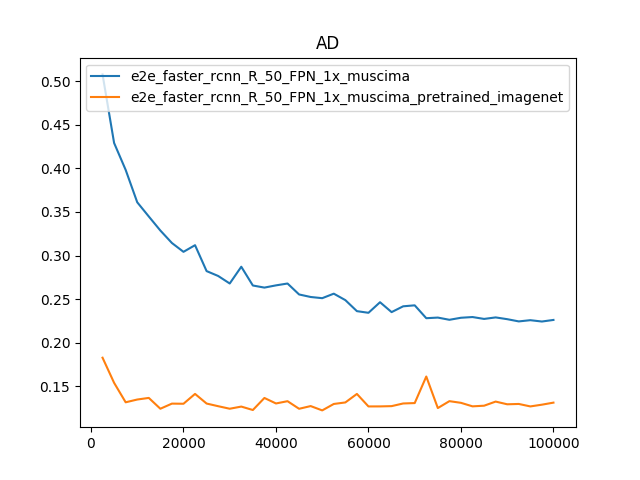
\includegraphics[width=3.8in]{img/AD.png}\\
			\caption{Comparing Average Distance between pretrained and non-pretrained network.}
			\label{fig:AD}
		\end{center}
	\end{figure}

	\subsection{Average Precisions}
	As regards the Average Precisions, similar results are observed: the AP of the pretrained model quickly grows to the maximum value, while the AP of the non-pretrained model grows slowly without reaching similar values to the other variant (Fig. \ref{fig:AP}, \ref{fig:AP50}, \ref{fig:AP75}).
	
	\begin{figure} [h]
		\begin{center}
			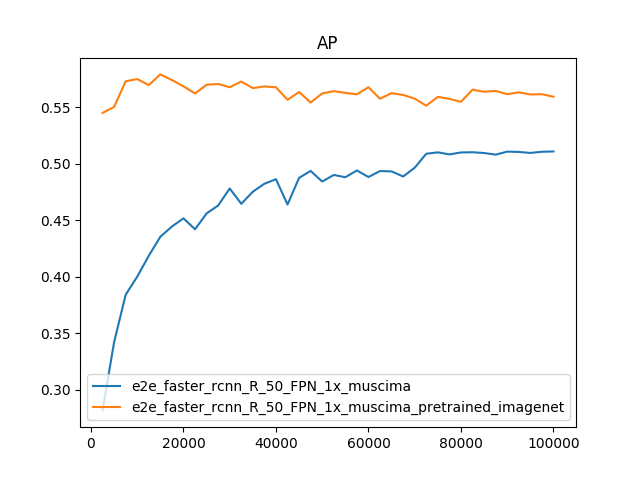
\includegraphics[width=3.8in]{img/AP.png}
			\caption{Comparing Average Precision between pretrained and non-pretrained network.}
			\label{fig:AP}
		\end{center}
	\end{figure}
	
	\begin{figure} [h]
		\begin{center}
			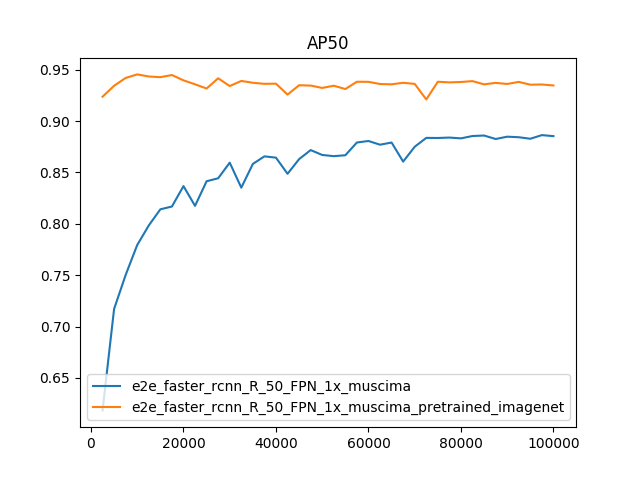
\includegraphics[width=3.8in]{img/AP50.png}
			\caption{Comparing Average Precision (considering boxes having at least IoU equal to 50) between pretrained and non-pretrained network.}
			\label{fig:AP50}
		\end{center}
	\end{figure}
	
	\begin{figure} [h]
		\begin{center}
			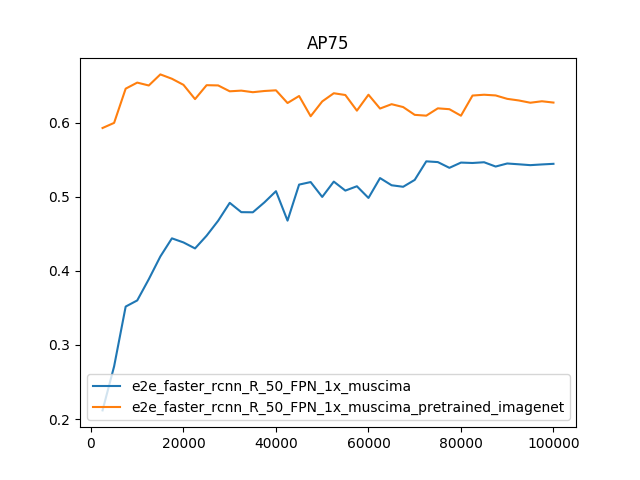
\includegraphics[width=3.8in]{img/AP75.png}
			\caption{Comparing Average Precision (considering boxes having at least IoU equal to 75) between pretrained and non-pretrained network.}
			\label{fig:AP75}
		\end{center}
	\end{figure}

	\section{Conclusions}
	We can see that the pretrained network reaches very quickly the best performances, a sign that transfer learning \cite{transfer-learning} works very well even in very different contexts. Instead, the non-pretrained network improves more slowly but continues to improve even after a long time, a sign that it needs more time to learn.
	
	However, we have obtained a good first result: it is possible to use standard object detection libraries for the notes detection in music sheets. Even if these libraries work better and are pretrained with common images with objects like people or cars, neural networks can learn to detect notes by their position inside the pentagram with good accuracy.
	
	\section{Future Works}
	There a lot of future possible works about OMR and particularly this project:
	\begin{itemize}
		\item Try a different backbone (like ResNet-101 or ResNet-152 \cite{RESNET}) to see if there are improvements.
		\item Extend the detection to all the notes, comprising also out of staffs notes.
		\item Define a better distance metric, considering how much the network is wrong (when it is).
		\item Use also distorted images offered by CVCMUSCIMA to improve network performances.
		\item Use data augmentation techniques to further enlarge the dataset.
	\end{itemize}
	
	\section*{Acknowledgment}
	The authors would like to thank Prof. Simone Marinai for the advice and the time spent with us during the project. 
	
	
	
	% if have a single appendix:
	%\appendix[Proof of the Zonklar Equations]
	% or
	%\appendix  % for no appendix heading
	% do not use \section anymore after \appendix, only \section*
	% is possibly needed
	
	% use appendices with more than one appendix
	% then use \section to start each appendix
	% you must declare a \section before using any
	% \subsection or using \label (\appendices by itself
	% starts a section numbered zero.)
	%
	
	% ============================================
	%\appendices
	%\section{Proof of the First Zonklar Equation}
	%Appendix one text goes here %\cite{Roberg2010}.
	
	% you can choose not to have a title for an appendix
	% if you want by leaving the argument blank
	%\section{}
	%Appendix two text goes here.
	
	
	% use section* for acknowledgement
	%\section*{Acknowledgment}
	
	
	%The authors would like to thank D. Root for the loan of the SWAP. The SWAP that can ONLY be usefull in Boulder...
	
	
	% Can use something like this to put references on a page
	% by themselves when using endfloat and the captionsoff option.
	\ifCLASSOPTIONcaptionsoff
	\newpage
	\fi
	
	
	
	% trigger a \newpage just before the given reference
	% number - used to balance the columns on the last page
	% adjust value as needed - may need to be readjusted if
	% the document is modified later
	%\IEEEtriggeratref{8}
	% The "triggered" command can be changed if desired:
	%\IEEEtriggercmd{\enlargethispage{-5in}}
	
	% ====== REFERENCE SECTION
	
	%\begin{thebibliography}{1}
	
	% IEEEabrv,
	
	\bibliographystyle{IEEEtran}
	\bibliography{IEEEabrv,Bibliography}
	%\end{thebibliography}
	% biography section
	% 
	% If you have an EPS/PDF photo (graphicx package needed) extra braces are
	% needed around the contents of the optional argument to biography to prevent
	% the LaTeX parser from getting confused when it sees the complicated
	% \includegraphics command within an optional argument. (You could create
	% your own custom macro containing the \includegraphics command to make things
	% simpler here.)
	%\begin{biography}[{\includegraphics[width=1in,height=1.25in,clip,keepaspectratio]{mshell}}]{Michael Shell}
	% or if you just want to reserve a space for a photo:
	
	% ==== SWITCH OFF the BIO for submission
	% mettere le foto nostre mi sembra pacchiano
	
	%% if you will not have a photo at all:
	%\begin{IEEEbiographynophoto}{Ignacio Ramos}
	%(S'12) received the B.S. degree in electrical engineering from the University of Illinois at Chicago in 2009, and is currently working toward the Ph.D. degree at the University of Colorado at Boulder. From 2009 to 2011, he was with the Power and Electronic Systems Department at Raytheon IDS, Sudbury, MA. His research interests include high-efficiency microwave power amplifiers, microwave DC/DC converters, radar systems, and wireless power transmission.
	%\end{IEEEbiographynophoto}
	
	%% insert where needed to balance the two columns on the last page with
	%% biographies
	%%\newpage
	
	%\begin{IEEEbiographynophoto}{Jane Doe}
	%Biography text here.
	%\end{IEEEbiographynophoto}
	% ==== SWITCH OFF the BIO for submission
	% ==== SWITCH OFF the BIO for submission
	
	
	
	% You can push biographies down or up by placing
	% a \vfill before or after them. The appropriate
	% use of \vfill depends on what kind of text is
	% on the last page and whether or not the columns
	% are being equalized.
	
	\vfill
	
	% Can be used to pull up biographies so that the bottom of the last one
	% is flush with the other column.
	%\enlargethispage{-5in}
	
	
	
	% that's all folks
\end{document}


